
%(BEGIN_QUESTION)
% Copyright 2012, Tony R. Kuphaldt, released under the Creative Commons Attribution License (v 1.0)
% This means you may do almost anything with this work of mine, so long as you give me proper credit

The Rosemount 3244MV FOUNDATION Fieldbus temperature transmitter is capable of receiving input signals from thermocouples, RTDs, and also generic millivoltage sources (over a range of -10 mV to +100 mV).  The option to input a millivoltage and digitally scale that analog signal into whatever range is desired is very useful.  Take for instance this application where we will use a Rosemount 3244MV transmitter to convert the signal from a tachogenerator into a speed indication for the motor (in units of RPM):

$$\includegraphics[width=15.5cm]{i01219x01.eps}$$

The tachogenerator is nothing more than a small, permanent-magnet DC generator whose output voltage is directly proportional to shaft speed (this one rated 10 volts output at 3000 RPM).

\vskip 10pt

Sketch a circuit connecting this tachogenerator to the 3244MV transmitter, ensuring the transmitter will never see more than 100 mV signal strength, and also determine the proper configuration parameters for this Fieldbus instrument's Analog Input (AI) block to scale the output so that it reports 0 to 2500 RPM:

% No blank lines allowed between lines of an \halign structure!
% I use comments (%) instead, so that TeX doesn't choke.

$$\vbox{\offinterlineskip
\halign{\strut
\vrule \quad\hfil # \ \hfil & 
\vrule \quad\hfil # \ \hfil \vrule \cr
\noalign{\hrule}
%
% First row
{\tt L\_Type} & \hskip 50pt \cr
%
\noalign{\hrule}
%
% Another row
{\tt XD\_Scale} & \hskip 50pt \cr
%
\noalign{\hrule}
%
% Another row
{\tt OUT\_Scale} & \hskip 50pt \cr
%
\noalign{\hrule}
} % End of \halign 
}$$ % End of \vbox

\vfil 

\underbar{file i01219}
\eject
%(END_QUESTION)





%(BEGIN_ANSWER)

This is a graded question -- no answers or hints given!

%(END_ANSWER)





%(BEGIN_NOTES)

This is just one possible solution:

$$\includegraphics[width=15.5cm]{i01219x02.eps}$$

% No blank lines allowed between lines of an \halign structure!
% I use comments (%) instead, so that TeX doesn't choke.

$$\vbox{\offinterlineskip
\halign{\strut
\vrule \quad\hfil # \ \hfil & 
\vrule \quad\hfil # \ \hfil \vrule \cr
\noalign{\hrule}
%
% First row
{\tt L\_Type} & Indirect \cr
%
\noalign{\hrule}
%
% Another row
{\tt XD\_Scale} & 0 to 83.33 mV \cr
%
\noalign{\hrule}
%
% Another row
{\tt OUT\_Scale} & 0 to 2500 RPM \cr
%
\noalign{\hrule}
} % End of \halign 
}$$ % End of \vbox

\vskip 10pt

Note that the {\tt OUT\_Scale} parameter is redundant in this application.  So long as {\tt L\_Type} is set to ``Direct'' the transmitter will report whatever its transducer senses, regardless of the {\tt OUT\_Scale} parameters.

%INDEX% Fieldbus, instrument ranging: setting XD_Scale and OUT_Scale parameters for an application

%(END_NOTES)


